\documentclass[a4paper]{article}

\usepackage[french]{babel}
\usepackage[utf8]{inputenc}
\usepackage{amsmath}
\usepackage{graphicx}
\usepackage{moreverb}
\usepackage{listings}
\usepackage[colorinlistoftodos]{todonotes}

\lstset{language=C++,
                basicstyle=\ttfamily\small,
                keywordstyle=\color{blue}\ttfamily,
                stringstyle=\color{red}\ttfamily,
                commentstyle=\color{gray}\ttfamily,
                morecomment=[l][\color{magenta}]{\#}
}

\title{Rapport d'implementation : Sparse Voxel DAG}

\author{Etienne Ferrier et Nikolai Morin}

\date{\today}

\begin{document}
\maketitle

\begin{abstract}
Ce rapport decrit notre implementation partielle du papier \textit{High Resolution Sparse Voxel DAGs} [Kämpe, Sintorn, Assarsson, 2013].
\end{abstract}

\section{Objectif de la publication originale}

Ce papier décrit comment construire, stocker et manipuler des Sparse Voxel Directed Acyclic Graphs (DAG) afin de décrire une scène de voxels. Les DAG sont une evolution des Sparse Voxel Octrees (SVO), qui permettent eux aussi de décrire une scène de voxels plus efficacement qu’une simple grille 3D.

Dans ce papier, les octrees et DAG sont utilisés en tant que que descripteurs d’une scène 3D et non seulement en tant que structures d’accélération.

L’intérêt des DAG est qu’ils permettent d’encoder l’information d'une scène de voxels de façon plus compacte qu’un SVO tout en ayant une structure efficace vis-à-vis des algorithmes de lancer de rayon.


\section{Implementation}

Grace a ce papier, nous avons implémenté :\\

\begin{itemize}
  \item Une structure inefficace \textit{pointer only} de SVO dont la manipulation est aisée et dont le parcours (lancer de rayons) est efficace.
  \item Une structure efficace \textit{mask-pointer} de SVO dont le stockage est reduit et dont le parcours est efficace.
  \item Une structure très compacte \textit{breath first} de SVO dont le stockage est très réduit mais dont le parcours est inefficace.
  \item Une structure efficace de DAG \textit{mask-pointer} dont le stockage est réduit et dont le parcours est efficace.
  \item Un algorithme qui permet de réduire un SVO en un DAG.\\
\end{itemize}

Nous avons pu comparer les résultats de ces différentes structures en termes de taille mémoire afin d'observer l'utilité des DAG.


Afin de comprendre toutes les étapes du pipeline du mesh au DAG, nous avons décidé de réaliser notre implémentation à partir du projet OpenGL de base du TD. Nous avons donc aussi implémenté notre propre conversion d’un 3D-mesh vers un SVO grâce à une méthode de lancer de rayons.

\begin{figure}
\centering
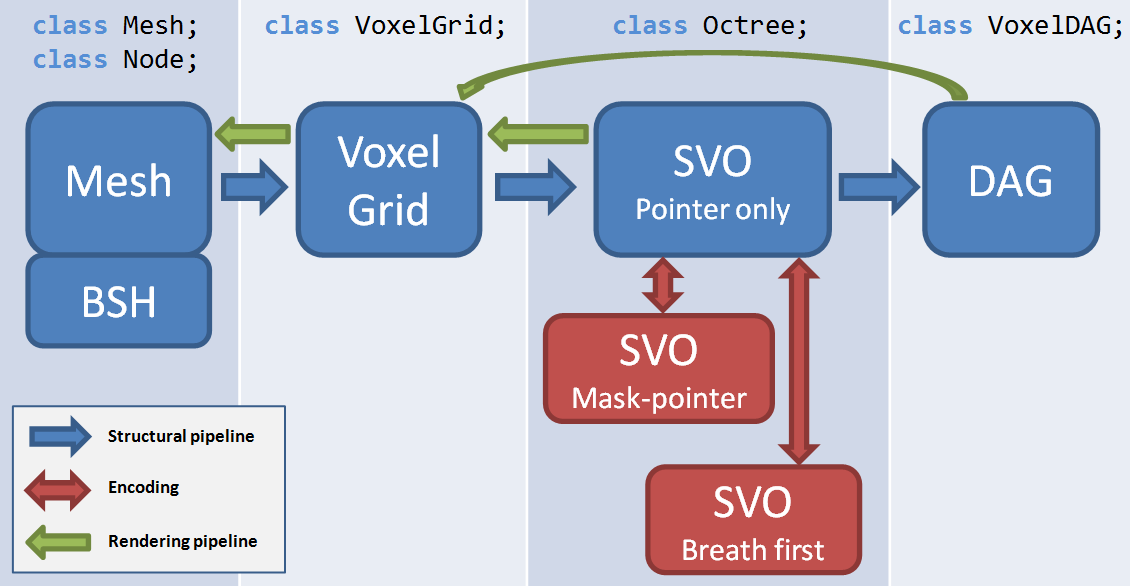
\includegraphics[width=1\textwidth]{ClassGraph.png}
\caption{\label{fig:triceratops}\textit{Pipeline of our implementation}}
\end{figure}

\subsection{SVO pointer only}

Nous utilisons la structure récursive suivante d’octree pour sa facilité de manipulation.

\begin{lstlisting}
class Octree {
	Octree* _childs; // = NULL ou Octree[8]
	bool _isEmpty;
};
\end{lstlisting}

Chaque nœud qui n’est pas une feuille (i.e qui ne représente pas un voxel) contient 8 pointeurs vers ses nœuds fils. La méthode \texttt{Octree::cutEmptyNodes();} permet d’en obtenir un SVO. 

\subsection{SVO mask-pointer}

La méthode suivante encode, pour chaque nœud d'un octree, un masque de 8 bits décrivant l’occupation de ses fils et un pointeur de 32 bits vers son premier fils non vide. 

\begin{lstlisting}
void Octree::encodeWithPointers(std::vector<uint8_t>& masks, 
	std::vector<int>& pointers, 
	std::vector<int>& levels);
\end{lstlisting}

Pour chaque nœud d'index i, son masque est stocké dans masks[i] et l’index de son premier fils non vide est stocké dans pointers[i].

\subsection{SVO breath-first}

La méthode suivante encode, pour chaque noeud, seulement un masque de 8 bits décrivant l’occupation de ses fils.

\begin{lstlisting}
void Octree::encodeBreadthFirst(std::vector<uint8_t>& storage);
\end{lstlisting}
 
Les nœuds sont listés dans l’ordre « largeur d’abord » dans le tableau storage.

\end{document}

